\documentclass{article}
\usepackage[margin=1in]{geometry}
\usepackage{amsmath}
\usepackage{amsfonts}
\usepackage{amssymb}
\usepackage{graphicx}
\usepackage{setspace}
\usepackage{tocloft}
\usepackage{subfiles}
\usepackage{multicol}
\usepackage{etoolbox,refcount}
\usepackage{subfiles}
\usepackage{titlesec}
\usepackage{float}
\title{COMP4901V Homework 2 Result}
\author{Leung Cheuk Wai 20771710}
\date{\today}

\begin{document}

\maketitle
\section*{2.1.1}
As the problem stated, the second camera is a pure translation that is parallel to the $x$-axis. So, the translateion can be written as :

\begin{equation*}
p_2 = T_x p_1
\end{equation*}

where $p_1$ and $p_2$ are corresponding points in two cameras, and $T_x$ is the translation matrix with pure translation that parallel to $x$-axis and $t$ in matrix represent the unit of translateion:

\begin{equation*}
T_x = \begin{bmatrix}
t & 0 & 0 \\
0 & 1 & 0 \\
0 & 0 & 1 \\
\end{bmatrix}
\end{equation*}

If we take a point $p_1$ in the first camera, its epipolar line in the second camera is given by:

\begin{equation*}
l_2 = F p_1
\end{equation*}

where $F$ is the fundamental matrix:

\begin{equation*}
F = K_2^{-T} T_x R K_1^{-1}
\end{equation*}
$R$ is an Identity matrix in this case as there are no rotation in this pure translation. So, 

\begin{align*}
    F &= K_2^{-T} T_x K_1^{-1}\\
T_x &= \begin{bmatrix}
    0 & 0 & 0 \\
    0 & 0 & -t \\
    0 & t & 0 \\
    \end{bmatrix}    
\end{align*} 

$K_1$ and $K_2$ are the camera calibration matrices for the two camera respectively where where $f_1$ and $f_2$ are the focal lengths, and $(c_{x_1}, c_{y_1})$ and $(c_{x_2}, c_{y_2})$ are the principal points of the two cameras.
\begin{equation*}
    K_n= \begin{bmatrix}
        f_n & 0 & c_{x_n}\\
        0 & f_n & c_{y_n}\\
        0 & 0 & 1\\
        \end{bmatrix}
\end{equation*}
Substituting the values of $T_x$ and $K_1$ and $K_2$, we get:
\begin{align*}
K_2^{-T} &= (K_2^{-1})^T = \begin{bmatrix}
    \frac{1}{f_2} & 0 & 0 \\
    0 & \frac{1}{f_2} & 0\\
    -\frac{c_{x_2}}{f_2} &  -\frac{c_{y_2}}{f_2} & 1 \\
    \end{bmatrix}\\
K_1^{-1}&=\begin{bmatrix}
    \frac{1}{f_1} & 0 & -\frac{c_{x_1}}{f_1} \\
    0 & \frac{1}{f_1} & -\frac{c_{y_1}}{f_1} \\
    0 & 0 & 1 \\
    \end{bmatrix}\\
F &= \begin{bmatrix}
    \frac{1}{f_2} & 0 & 0 \\
    0 & \frac{1}{f_2} & 0\\
    -\frac{c_{x_2}}{f_2} &  -\frac{c_{y_2}}{f_2} & 1 \\
    \end{bmatrix}
    \begin{bmatrix}
    0 & 0 & 0 \\
    0 & 0 & -t \\
    0 & t & 0 \\
    \end{bmatrix}
    \begin{bmatrix}
    \frac{1}{f_1} & 0 & -\frac{c_{x_1}}{f_1} \\
    0 & \frac{1}{f_1} & -\frac{c_{y_1}}{f_1} \\
    0 & 0 & 1 \\
    \end{bmatrix} \\
&= \begin{bmatrix}
    0 & 0 & 0 \\
    0 & 0 & -\frac{t}{f_2} \\
    0 & t & t\frac{c_{y_2}}{f_2} \\
    \end{bmatrix}
\begin{bmatrix}
    \frac{1}{f_1} & 0 & -\frac{c_{x_1}}{f_1} \\
    0 & \frac{1}{f_1} & -\frac{c_{y_1}}{f_1} \\
    0 & 0 & 1 \\
    \end{bmatrix}\\
&= \begin{bmatrix}
    0 & 0 & 0 \\
    0 & 0 & -\frac{t}{f_2}\\
    0 & \frac{t}{f_1} & \frac{tc_{y_2}}{f_2}-\frac{tc_{y_1}}{f_1} \\
    \end{bmatrix}
\end{align*}

So,  the epipolar line in camera 2 corresponding to a point $p_1$:
\begin{align*}
    l_2 &= F p_1 \\
    &= \begin{bmatrix}
        0 & 0 & 0 \\
        0 & 0 & -\frac{t}{f_2}\\
        0 & \frac{t}{f_1} & \frac{tc_{y_2}}{f_2}-\frac{tc_{y_1}}{f_1} \\
        \end{bmatrix} \begin{bmatrix}
    x_1 \\
    y_1 \\
    1 \\
    \end{bmatrix}\\
    & =  \begin{bmatrix}
        0 \\
        -\frac{t}{f_2} \\
        \frac{y_1 t}{f_1}+\frac{tc_{y_2}}{f_2}-\frac{tc_{y_1}}{f_1}\\
        \end{bmatrix}
\end{align*}
The second coordinate is constant, so the epipolar line is parallel to $x$-axis in the second camera. Similarly, the first camera did the same work. So, we can conclude that the epipolarlines in both camera is parallel to $x$-axis

\section*{2.1.2}
Effective rotation and translation between two frames at different time stamps:
\begin{align*}
R_{rel} &= R_{2} R_{1}^T \\
t_{rel} &= t_{2} - R_{rel} t_{1} \\
\end{align*}

Essential matrix:
\begin{equation*}
%E = K^T \begin{bmatrix} 0 & -t_{rel,z} & t_{rel,y} \\ t_{rel,z} & 0 & -t_{rel,x} \\ -t_{rel,y} & t_{rel,x} & 0 \end{bmatrix} R_{rel} K
E = [t_{rel}]\times R_{rel}
\end{equation*}

Fundamental matrix:
\begin{equation*}
F = K^{-T} [t_{rel}]\times R_{rel} K^{-1}\end{equation*}
\section*{2.1.3}
The reflection point of $x$ is $x'$=$R_fx$, where $R_f$ is the reflection.\\
$R_f$=$H\begin{bmatrix}
    \Lambda &0\\
    0^T &1\\
\end{bmatrix}H^-1$ and $H=\begin{bmatrix}
    R&t\\
    0&1
\end{bmatrix}$ and $\Lambda=\begin{bmatrix}
    -1&0&0\\
    0&1&0\\
    0&0&1
\end{bmatrix}$\\
At Camera $C$, the points will be $C_x$ and $C_x'$=$C R_f x$ which is equivalent to $x$ by two camera $C$ and $CR_f$\\
\begin{align*}
    C&=K[I|0]\\
    CR_f&=K[I|0]H\Lambda H^-1\\
    &=K[R\Lambda R^T|-R\Lambda R^Tt]\\
    &=K[R\Lambda R^T|R\Gamma R^Tt]\\
\end{align*}
where \begin{equation*}
    \Gamma=I-\Lambda=\begin{bmatrix}
        2&0&0\\
        0&0&0\\
        0&0&0
    \end{bmatrix}
\end{equation*}
The corresponding canonical cameras are $[I|0]$ and $K[R\Lambda R^T|R\Gamma R^Tt]$.\\
From previous part, we got 
    $F = K^{-T} [t_{rel}]\times R_{rel} K^{-1}$
    where $t_{rel}$ is the relative translation between the two cameras and $R_{rel}$ is the relative rotation matrix.

    We can rewrite $F$ in terms of the two cameras $C$ and $CR_f$ as follows:
    
    \begin{align*}
    F &= K^{-T} [t_{rel}]\times R_{rel} K^{-1}\\
    &= K^{-T} [R\Gamma R^Tt]\times R K^{-1}\\
    &= K^{-T} [R\Gamma R^Tt]\times R K^{-T} K K^{-1}\\
    &= K^{-T} [R\Gamma R^Tt]\times R K^{-T} C^{-1} CR_f^{-1}\\
    &= (CR_f^{-T})^{-1} \begin{bmatrix} R\Gamma R^Tt \end{bmatrix}\times (CR_f^{-1})^{-1}\\
    &= \begin{bmatrix} CR_f^{-T}t\times R\Gamma R_f^{-1} \end{bmatrix}_\times\\
    \end{align*}
    
    where $t_\times$ is the skew-symmetric matrix associated with the translation vector $t$. We can see that $F$ is skew-symmetric, which is a necessary condition for it to be a fundamental matrix.
    
    Therefore, we have shown that the situation where a camera views an object and its reflection in a plane mirror is equivalent to having two images of the object which are related by a skew-symmetric fundamental matrix $F$.
    \section*{2.3.1}

    \begin{figure}[H]
        \centering
              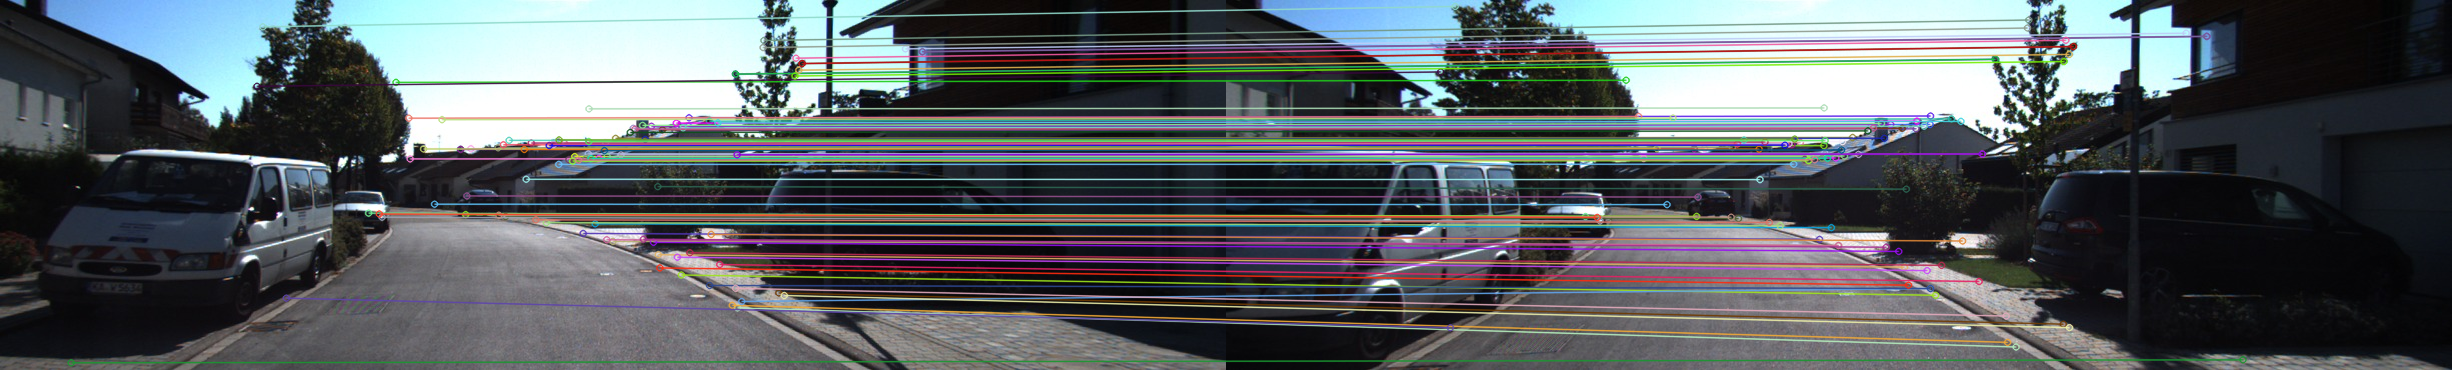
\includegraphics[width=0.8\linewidth]{../homework/2_3_1_fig1.png}
              \label{figure3}
    \end{figure}
    \section*{2.3.2}
    
    F=$\begin{bmatrix}
        -1.41020931e-06&2.47964903e-06&2.78876008e-04\\
        2.16115677e-06&-6.16791447e-06&1.02702596e-04\\
        2.14053286e-04&-2.77064401e-04&-6.45640986e-02
    \end{document}